\section{Problema de planificación de producción tipo taller (JSSP)}
Una instancia del JSSP consiste en $n$ trabajos diferentes constituidos cada uno por $m$ operaciones que deben procesarse por un tiempo determinado en $m$ máquinas en una secuencia predeterminada.\\
El objetivo es hallar la planificación que minimiza el tiempo que toma terminar todos los trabajos dado que cada máquina puede procesar solo un trabajo a la vez.

Una planificación consiste en asignar tiempos de inicio y fin a cada operación respetando el orden requerido para cada trabajo. El tiempo que toma terminar todos los trabajos se conoce como makespan y la secuencia de trabajos que toma el mayor tiempo en completarse se conoce como ruta crítica. La ruta crítica puede verse como una serie de bloques críticos que consisten en las secuencias de operaciones de la ruta crítica que se ejecutan de forma adyacente en la misma máquina. Una planificación puede tener una o varias rutas críticas. \\
Sin pérdida de generalidad podemos restringirnos al caso en el que el tiempo requerido para procesar cada operación es un entero positivo.\\

\subsection*{Ejemplo}
Se muestra un ejemplo de una instancia con 3 máquinas y 2 trabajos.
\begin{table}[H]
\centering
\caption{Instancia simple con 3 maquinas y 2 trabajos}
\begin{tabular}{@{}llll@{}}
Trabajo & \multicolumn{3}{l}{\begin{tabular}[c]{@{}l@{}}Secuencia de procesamiento \\ (máquina, tiempo)\end{tabular}} \\ \midrule
0       & 0, 75                              & 2, 54                               & 1, 59                             \\ \midrule
1       & 0, 47                              & 2, 72                              & 1, 45   \\\hline                         
\end{tabular}
\label{tab:inst}
\end{table}

La siguiente es una posible planificación para la instancia de ejemplo, visualizada mediante un diagrama de gantt. En negro se marca los trabajos que conforman la ruta crítica. 
\begin{figure}[H]
\centering
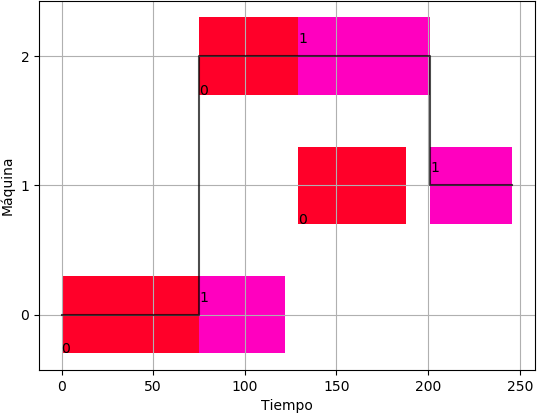
\includegraphics[scale=.7]{Imagenes/planejemplorc.png}
\caption{Diagrama de gantt de una planificación posible}
\label{fig:gantt}
\end{figure}


\section{Representación de planificaciones}
Existen varias formas de representar las planificaciones, en este trabajo se utilizaron dos: el grafo disyuntivo y las reglas de prioridad.
\subsection*{Modelo de grafo disyuntivo} 
En este modelo las planificaciones se representan con un grafo dirigido $G=(V,A,E)$ en el que $V$ es un conjunto de nodos que representa las operaciones, las aristas $A$ representan la secuencia que deben seguir las operaciones dentro de un mismo trabajo y $E$ es otro conjunto de aristas que indica el orden de procesamiento en cada una de las máquinas. Es importante mencionar que con este modelo podemos representar planificaciones no factibles, esto se da cuando el grafo $G$ contiene un ciclo.


Formalmente en una instancia del JSP se representa cada operación como un nodo, se agregan dos nodos de control que sirven como el nodo inicial (del que dependen todos los trabajos) y final (que depdende de todos los trabajos), las restricciones de precedencia dentro de cada trabajo se representan como aristas dirigidas fijas llamadas aristas conjuntivas y las operaciones que deben procesarse en una misma máquina se unen mediante aristas llamadas disyuntivas, una solución factible o planificación se obtiene al elegir la dirección para cada arista disyuntiva de modo que no se generen ciclos.   
%El problema de hallar una planificación para cada una de las $m$ operaciones de los $n$ trabajos en las $m$ máquinas se reduce a elegir una permutación de los $n$ trabajos en cada máquina por lo que el número de posibles soluciones es $O(n!^m)$.

% poner las representaciones
\begin{figure}
\centering
\subfigure[Representación de una instancia, los colores distinguen entre las tres máquinas.]{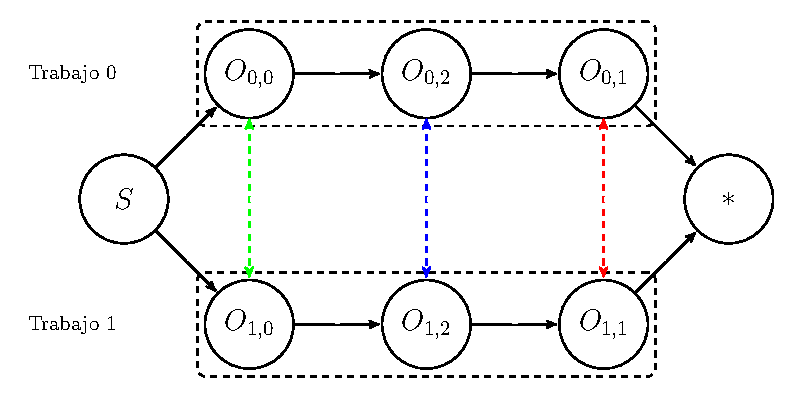
\includegraphics[scale=.7]{Imagenes/disyuntive.pdf}}
    \subfigure[Planificación obtenida al fijar las aristas disyuntivas como en \ref{fig:gantt}. La ruta critica se resalta en amarillo]{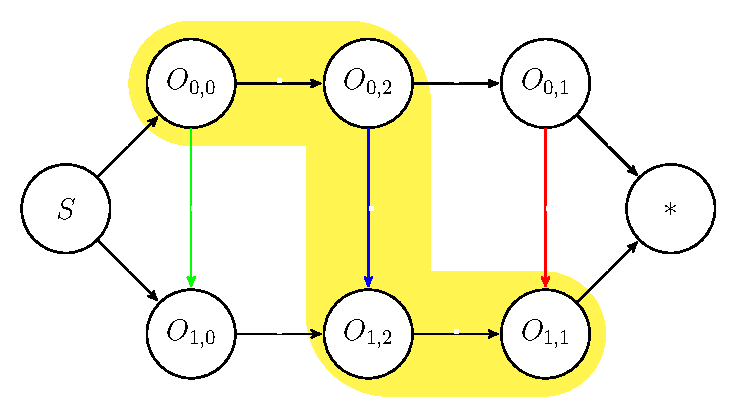
\includegraphics[scale=.7]{Imagenes/plandisyuntive.pdf}}
\caption{Modelo de grafo disyuntivo para la instancia de ejemplo \ref{tab:inst}}
\end{figure}

\subsection*{Reglas de prioridad}
En esta representación una planificación se construye al aplicar un proceso de simulación en el que para cada maquina se construye una cola con las operaciones cuyas dependencias ya han sido procesadas. Inicialmente se tienen en las colas solo las operaciones iniciales de cada trabajo. Una vez que se tiene esto se utiliza una regla de prioridad para elegir qué operación debe planificarse en qué máquina. Se actualizan las colas para las máquinas que lo requieran y se continua con este proceso hasta completar la planificación (vaciar las colas).

Existen muchas reglas de prioridad que toman en cuenta cosas como la duración de la operación, la cantidad de operaciones restantes, la duración del trabajo al que pertenece una operación, entre muchas otras. La calidad de la planificación construida depende de la regla de prioridad que se utilice y de la estructura de la instancia en sí.


\section{Tipos de planificaciones}
Independientemente de cómo se representen o como se construyan las planificaciones pueden clasificarse en varios conjuntos. Dentro de el conjunto de planificaciones factibles se pueden distinguir dos subconjuntos de interés para el presente trabajo: el conjunto de las planificaciones óptimas que está conformado por las planificaciones con el menor makespan posible y el conjunto de las planificaciones activas. 
Estas últimas se definen como las planificaciones en las que no es posible disminuir el tiempo de inicio de ninguna operación sin aumentar el tiempo de inicio de otra. Es conocido que las planificaciones óptimas representan un subconjunto de las activas\cite{Ponsich2013}.

% imagen 

\begin{figure}[H]
    \centering
    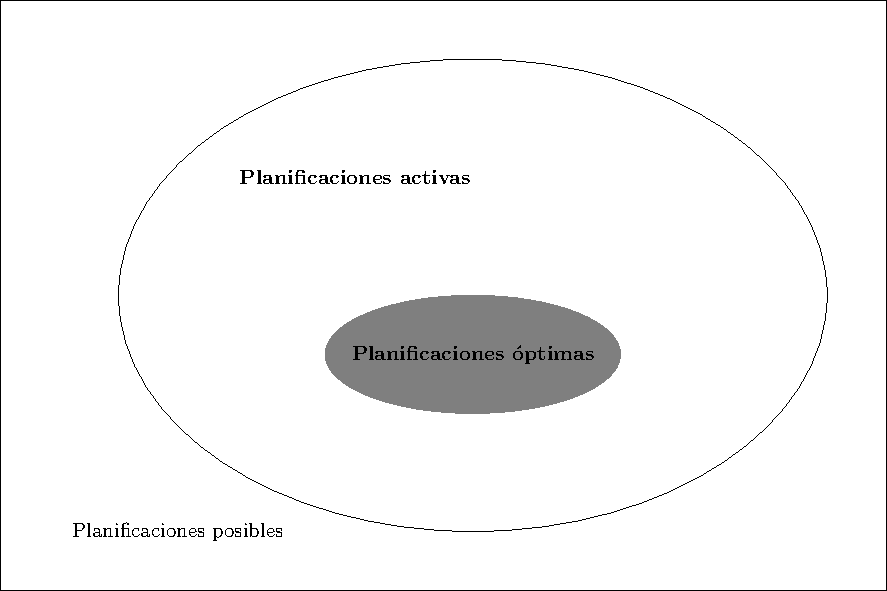
\includegraphics[scale=.8]{Imagenes/solspace.pdf}
    \caption{Subconjuntos de planificaciones}
\end{figure}

Estas clasifaciones resultan interesantes porque existen algoritmos para generar tipos de planificaciones de modo que podamos centrarnos en solo un subconjunto del espacio de búsqueda.
